
% 学位论文的正文应以《绪论》作为第一章
\chapter{绪论}\label{chapter_introduction}
\section{研究背景}

近年来,人工智能领域的深度学习技术在各个应用领域都获得了迅速的发展。依赖于大数据时代数据量的爆发式增长,以及高性能计算设备的不断发展,深度神经网络(deep neural networks, DNN)在推荐系统 \upcite{recomendation1,recomendation2},图像识别 \upcite{resnet, imagenet, amoebanet}, 物体检测\upcite{yolo, yolov3} 以及自然语言处理 \upcite{bert,bart} 等应用领域都进行了广泛的应用,并且取得了巨大成功。

如图 \ref{fig:dnn-arch}所示,典型的深度神经网络由若干算子(卷积、池化、全连接等)搭建而成,不同的算子构建成层状结构,层与层被连接在一起,最终构成完整的神经网络模型。
深度神经网络主要依赖反向传播算法 (Back propagation) \upcite{bp}进行训练。以图像识别任务为例,在进行训练前,首先需要将模型的参数加载到内存中,然后针对训练数据,分批次迭代式的读取训练数据和数据对应的标签,首先经过前向传播,将数据输入到模型中,得到模型预测结果。然后将模型预测结果和真实标签输入到损失函数中,计算出损失,再进行反向传播,求解模型参数关于损失的梯度。得到梯度后,再根据优化器 \upcite{adam,rmsprop}的优化策略,对模型参数进行优化。重复上述过程,直到模型收敛。
从反向传播算法的运行过程可以看出,深度神经网络模型的训练是计算密集型任务,训练过程中需要涉及到高维数据的处理,反向传播求导,以及参数优化等。因此,目前的深度神经网络模型的训练通常需要使用专用的高性能计算设备来进行,例如GPU,TPU以及FPGA等 \upcite{tpu-gpu}。
\begin{figure}[h]
	\centering
	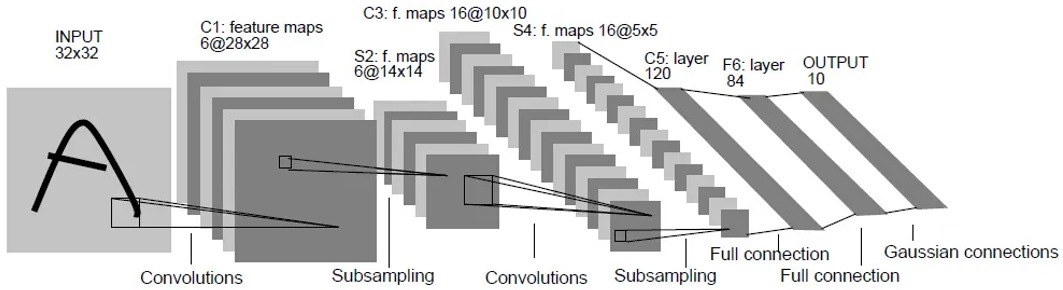
\includegraphics[width=0.8\textwidth]{figure/1-intro/dnn.png}
	\caption{典型深度神经网络结构}
	\label{fig:dnn-arch}
\end{figure}

以深度神经网络为代表的深度学习技术在性能提高的同时,也伴随着模型大小的增加和模型结构复杂度的提升。
以目前主流的高性能计算设备GPU为例,单个设备,无论是运算性能还是设备内存大小,都无法满足模型的训练需求,因此,使用多个设备进行训练,以提升训练效率,已经成为了深度学习领域的最佳实践。
如图 \ref{fig:model-mem} 所示,如果我们使用主流的ResNet-152模型,以$224\times 224$分辨率的输入,在32位浮点精度下,去训练图像识别任务,那么当数据批的大小达到$128$时,就会超过40GB的显存用量,此时,单个GPU设备的显存容量已经很难满足需求。

\begin{figure}[h]
    \centering
    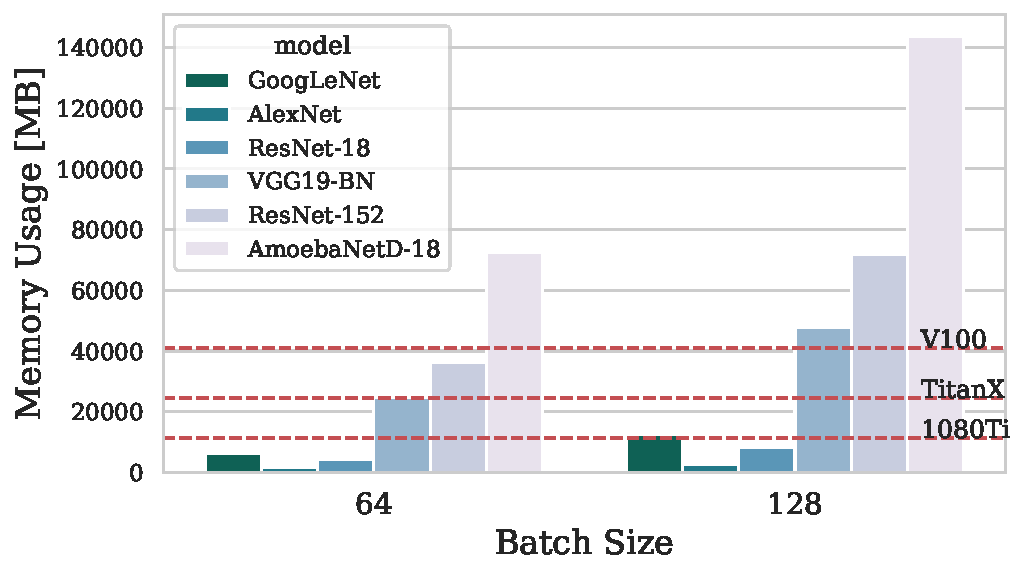
\includegraphics[width=0.8\textwidth]{figure/1-intro/model_mem.pdf}
    \caption{主流计算机视觉模型显存消耗}
    \label{fig:model-mem}
\end{figure}

另一方面,数据集的大小也在不断增大。以ILSVRC-ImageNet2012 \upcite{imagenet} 为例,该数据集的训练集包括1000个分类类别,1300万张训练图片,训练集总大小超过120GB。如果使用单个设备进行训练,将所有图片训练一次(Epoch)需要超过数个小时的时间,而训练需要迭代式进行,往往需要经过多个轮次才能收敛,因此,使用多个计算设备加速训练过程是必要的。

综上所述,使用多个计算设备进行模型训练可以带来以下两点好处:
\begin{itemize}
	\item \textbf{允许训练更大的模型}: 受限于访存速度和制造成本,单个GPU设备的内存容量是有限的。针对大模型,模型的参数会占据大量内存空间,导致没有充足的内存空间去存储训练过程的中间结果、参数梯度等。而对于超大模型,甚至模型参数本身所使用的内存空间就会超过单个设备的内存容量。因此对于这类超大型深度神经网络模型(Giant DNN),使用多个设备进行协同训练是十分必要的。
	\item \textbf{提升训练效率}:模型训练通常使用批处理的方式进行训练,利用GPU的并行计算能力,同时处理一个数据批(Data batch)可以有效加速模型的训练速度,另一方面,使用数据批可以减少对模型参数进行梯度下降优化时的方差,加快收敛速度,现有工作 \upcite{large-batch} 表明,使用大数据批可以更好的代表样本总体,让模型准确的找到收敛方向。而使用大数据批的前提是需要有可用的显存空间,而使用多个GPU设备可以提供更多显存,从而允许算法研究者使用更大的数据批进行训练,提升训练效率,加快模型收敛速度。
\end{itemize}

随着深度学习的不断发展,使用多个设备加速深度神经网络的训练已经成为了最佳实践。
目前主流的开源机器学习框架,如PyTorch \upcite{pytorch} , Tensorflow\upcite{tensorflow} , MXNet\upcite{mxnet} 等,也提供了对多设备并行训练的支持,但是目前,对于超大模型的训练,主流框架多依赖于使用者对多设备协作训练进行手动配置,缺少对于超大模型训练的自动化支持。
尤其是在异构计算集群中,即使对于有经验的算法研究者,也无法总是准确考虑集群中的异构性,设备之间的通信特征以及模型的特点,这导致人工给出的模型训练配置往往不能很好的提高硬件利用率,达到最佳训练效率。因此,设计一种能够自动化完成超大模型端到端训练,自动进行模型划分,多设备协作的训练框架是十分有必要的。


\section{研究现状}
% 
目前,随着各种超大模型被设计出来,利用多设备去并行训练模型,加快模型训练速度的分布式深度学习 \upcite{ddl-survey}成为了机器学习领域的一个重要分支。
针对不同的场景,分布式深度学习有着不同的发展方向。目前,分布式深度学习有三种主要分支:
\begin{itemize}
	\item \textbf{数据并行化 (Data Parallelism, DP)}:数据并行化关注数据吞吐量的提升,也就是单位时间内,模型能够训练的数据样本数目。在数据并行化中,通常存在多个被称作Worker的计算单元,每个Worker使用一个设备,多个Worker之间进行协作完成训练。每个设备持有一个完整的模型副本,Worker使用不同的数据训练本地的模型,并按照一定的策略同步本地模型的参数,这就是数据并行化的思路。
	\item \textbf{模型并行化 (Model Parallelism, MP)}:针对超大模型在单个设备上训练受限的问题,模型并行化被提出,模型并行化也是本文研究的重点。与数据并行化不同,模型并行化针对如何将大型模型划分到多个设备上进行训练,每个设备只持有部分模型,反向传播算法在设备之间分布式运行,设备之间通过通信去传递中间结果以及反向传播过程中产生的梯度。在模型并行化中,由于每个设备只负责部分模型的训练,所以需要按照某些规则对模型进行划分,在划分时,需要考虑设备的负载均衡,避免某个设备的负载较大,成为瓶颈。另一方面,由于模型并行化中,设备之间需要进行大量通信,因此在划分时,也要考虑通信数据量、设备之间的通信链路对于训练效率的影响。
	\item \textbf{混合并行化 (Hybrid Parallelism, HP)}:混合并行化结合数据并行化和模型并行化二者的优势,先将超大模型划分为多个部分,每个部分由若干Worker构成的组进行训练,组内使用数据并行化,加大数据吞吐,组与组之间使用模型并行化,由于结合了二者的优点,因此混合并行化也是针对大模型使用的比较多的一种训练方式。
\end{itemize}

在模型并行化中,由于不同设备之间存在依赖关系,因此设备之间存在互相等待的现象,导致设备利用率低,针对这一问题,研究者专注于设计更好的通信模式,通过流水线的方式,让设备的计算过程和设备之间的通信过程重叠,从而提高设备利用率\upcite{gpipe,pipedream,hetpipe,hippie,dapple}。
Huang \upcite{gpipe} 等人提出了Gpipe技术,通过将数据批进一步细分成更小的微数据批(micro batch),将模型并行化以流水线的形式构建,加速模型并行化训练。
Narayanan \upcite{pipedream} 等人提出了PipeDream,在模型并行化流水线中引入异步计算,在内存中维护了多个版本的模型参数,以空间换时间,进一步提升训练效率。

除了使用流水线技术去改善模型并行化的训练效率外,模型并行化领域的另一个问题是,针对超大模型如何进行模型的划分 \upcite{rl1,rl2,baechi,pesto,rannc}。
Mirhoseini \upcite{rl1,rl2} 等人提出利用强化学习技术进行模型划分,但是随着模型大小的增加和模型复杂度的提升,强化学习收敛慢的问题在面对超大模型时变得更为突出。
Jeon \upcite{baechi} 等人将模型划分问题抽象为处理器调度问题,使用经典的任务调度算法,对模型进行划分。
相比于强化学习,尽管Jeon所使用的任务调度算法运行速度更快,但是其使用的算法是近似算法,在通信受限的场景下近似比较大,无法获得较优的结果。
Hafeez \upcite{pesto} 等人将模型划分问题进行建模,并利用线性规划进行求解。但是该工作只考虑了设备数目为2的简单情况,没有扩展到更多数目的设备,并且在进行问题建模时,没有考虑反向传播开销的影响。

综上所述,现有的模型划分方法仍然存在缺陷,使用模型并行化去训练超大模型时,如何去划分和放置模型仍然是一个亟待解决的问题。

\section{本文工作}
% 实现了xxx系统,使用xxx技术,解决了xxx问题
本文设计并实现了\sys,一种可以进行自动化模型划分与设备放置的超大型神经网络训练框架。
针对神经网络的模型划分问题,\sys 没有对神经网络进行粗粒度的分层切分,而是从神经网络底层的计算图出发,通过将原始模型转换成一种计算图的中间表示,以图的节点为单位对计算图进行细粒度的划分,并从划分后的计算图中重建出与原始模型等价的模型。
为了实现更好的划分效果,\sys 首先对训练使用的硬件环境进行性能测试,主要测试参与训练的设备之间的点对点通信带宽。
接着\sys 会对模型计算图进行分析,通过动态分析和静态分析的方法,获取计算图上每个节点的前向传播用时、反向传播用时、显存用量等模型元信息。
获取元信息之后,\sys 构建出模型划分与设备放置的约束优化问题,以提升训练效率为优化目标,进行求解。
求解完成后,\sys 将划分后的计算图按照求解结果进行设备放置,并基于PyTorch\upcite{pytorch} 实现后续的训练过程。

综上所述,本文提出了一种针对超大型神经网络模型的训练框架\sys,其主要的工作包括:
\begin{itemize}
	\item 基于开源机器学习框架PyTorch,实现了一种可以自动对通用PyTorch模型进行模型划分、设备放置以及训练的框架,可以有效解决大型神经网络在单个设备上难以训练的问题。
	\item \sys 可以根据训练任务所使用的硬件环境,自动化的对硬件进行点对点带宽测试,充分考虑模型并行化任务中,设备之间的通信链路对模型划分效果的影响。
	\item \sys 中实现了一种可以自动将通用的PyTorch模型转化成一种计算图中间表示的功能模块,基于这种计算图的中间表示,\sys 以计算图节点为粒度进行模型划分,相比于以层为粒度进行模型划分,更加细粒度,且更加通用。
	\item 设计了详细的对比实验:分别针对图像分类和图像分割两种任务,选用包括Wide-ResNet152\upcite{resnet} , AmoebaNetD-18\upcite{amoebanet}, U-Net\upcite{unet} 和DeepLab-V3\upcite{deeplabv3}在内的大模型,将\sys 与多种现有的模型划分与设备放置方法进行对比。实验结果显示,相比于现有方法,在不同模型上,\sys 的对于模型训练效率具有至少$4.4\% \sim 14.82\%$的提升。
\end{itemize}

\section{本文组织}
本文剩余章节组织如下:

第二章介绍与本文研究方向相关的技术背景和工作。
首先将介绍本文中出现的一些术语,然后会介绍主流的分布式深度学习技术与发展现状,模型并行化技术的发展,现有的模型划分技术,以及模型训练与计算图方面的工作,并分析大型神经网络模型训练中的难点和挑战。

第三章介绍我们针对大型神经网络模型训练设计的训练框架\sys 以及\sys 中各个功能模块的实现,包含模型转换模块、模型分析模块(显存/计算用时)、通信代价建模模块、计算图划分模块以及最后的模型训练模块。

第四章介绍\sys 中核心算法的实现细节,包括对问题的形式化描述、计算图优化算法、计算图划分算法等。

第五章对\sys 与其他模型划分与设备放置算法的实验进行详细介绍。包括实验对比方法、实验的硬件设置、实验的指标以及实验结果的分析。

第六章对本文工作进行总结,对当前工作中的不足进行分析,并展望本文工作未来的发展。